\documentclass{article}
\usepackage[T1]{fontenc}
\usepackage{lmodern}
\usepackage{graphicx}
\usepackage{amsmath,amssymb}
\usepackage[a4paper,margin=2cm]{geometry}
\usepackage[absolute,overlay]{textpos}
\setlength{\TPHorizModule}{1mm}
\setlength{\TPVertModule}{1mm}
\usepackage[indonesian]{babel}
\usepackage{hyperref}
\setlength{\emergencystretch}{2em}
% unit: Halaman 20

\begin{document}

% === Halaman 20 (llm) ===

\section*{Pelelaran Titik}

\vspace{160.38mm}

\begin{itemize}
    \item Pelelaran titik (\textit{point iteration}): menjumlahkan sebuah titik sebanyak $k - 1$ kali terhadap dirinya sendiri.
    \item $P^k = kP = P + P + \dots + P$
    \item Jika $k = 2 \rightarrow P^2 = 2P = P + P$
\end{itemize}

\vspace{20mm}

\textcolor{red}{\text{Sumber gambar: Andreas Steffen, Elliptic Curve Cryptography}}

% deskripsi: Grafik ilustrasi operasi pelelaran titik pada kurva eliptik yang menunjukkan titik P, P^2, dan P^3 serta garis bantu yang digunakan dalam proses penjumlahan titik.
% bbox normalisasi: [0.5100, 0.3700, 0.8400, 0.9100]
\begin{textblock*}{69.30mm}(107.10mm,109.89mm)
\noindent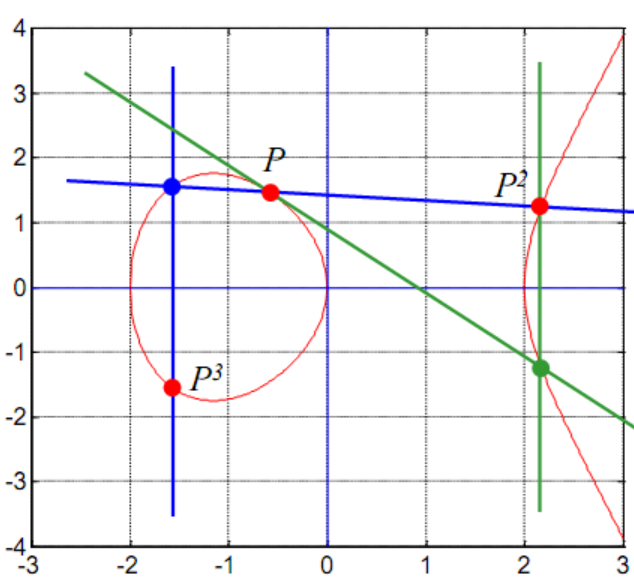
\includegraphics[width=69.30mm,height=160.38mm]{../../images/llm/page_020_img_01.png}%
\end{textblock*}

\end{document}
